\appendix
\section*{Appendix}
\appendixtoc
\clearpage

\newenvironment{longlisting}{\captionsetup{type=listing}}{}

\section{Source Code}

\vspace{1em}

\begin{longlisting}
\begin{minted}[frame=lines, fontsize=\scriptsize, baselinestretch=1]{md}
> Eine Nudel is ein – also n ganz‘ Tach.
> Man kann im Winter Sommer,
> Man kann morgens abends essen,
> ein Nudel is wirklich ein sehr leckeres Gericht.
>
> Man kann Nudeln machen warm,
> man kann Nudeln machen kalt.
> Also man kann in den Urlaub,
> man kann nen Picknick machen,
> man kann abends morgens essen,
> wie man gerade Hunger hat.
>
> Dawegen spielt’s keine Tageszeit,
> keine Sonnenzeit, kein Winter oder so –
> die Italiener essen es auch jeden Tach.
> Also ist eine Nudel ein ein ein ewig’s Essen.
>
> Egal aus was ist die Nudel gemacht ist,
> egal wie Du Nudel zubereitet wird.
> Jeder hat seinen Geschmack,
> einer ist gerade morgens aufgestanden
> ist – äh – gerne Nudeln
> der macht sich auch morgens Nudeln –
> kein bisschen…
>
> Dawegen lass ich auf Nudeln nix kommen
> Humor muss sein.
> Dafür ist ja die humorvolle italienische Nudeln,
> der hat ja auch Humor der Italiener.
>
> Eine Nudel kräftigt –
> eine Nudel kräftigt nicht nur,
> die hat Energie bringt sie,
> auch nich dann noch dafüchtüch
> wenn man die gegessen hat,
> hat man auch Freude an den ganzen Tag
> um so schneller ist man, oder –
> umso mehr baut man seine Kraft –
> und seine Freude auf.
>
> Das ist das Wichtige, ha haaa!
>
> Die Nudel schmeckt, dadrauf kommts an.
\end{minted}
  \caption{Peter Ludolfs "Ode an die Nudel"}
  \label{lst:ludolf-nudel}
\end{longlisting}

\section{Non-Disclosure Note}

\begin{figure}[H]
  \centering
  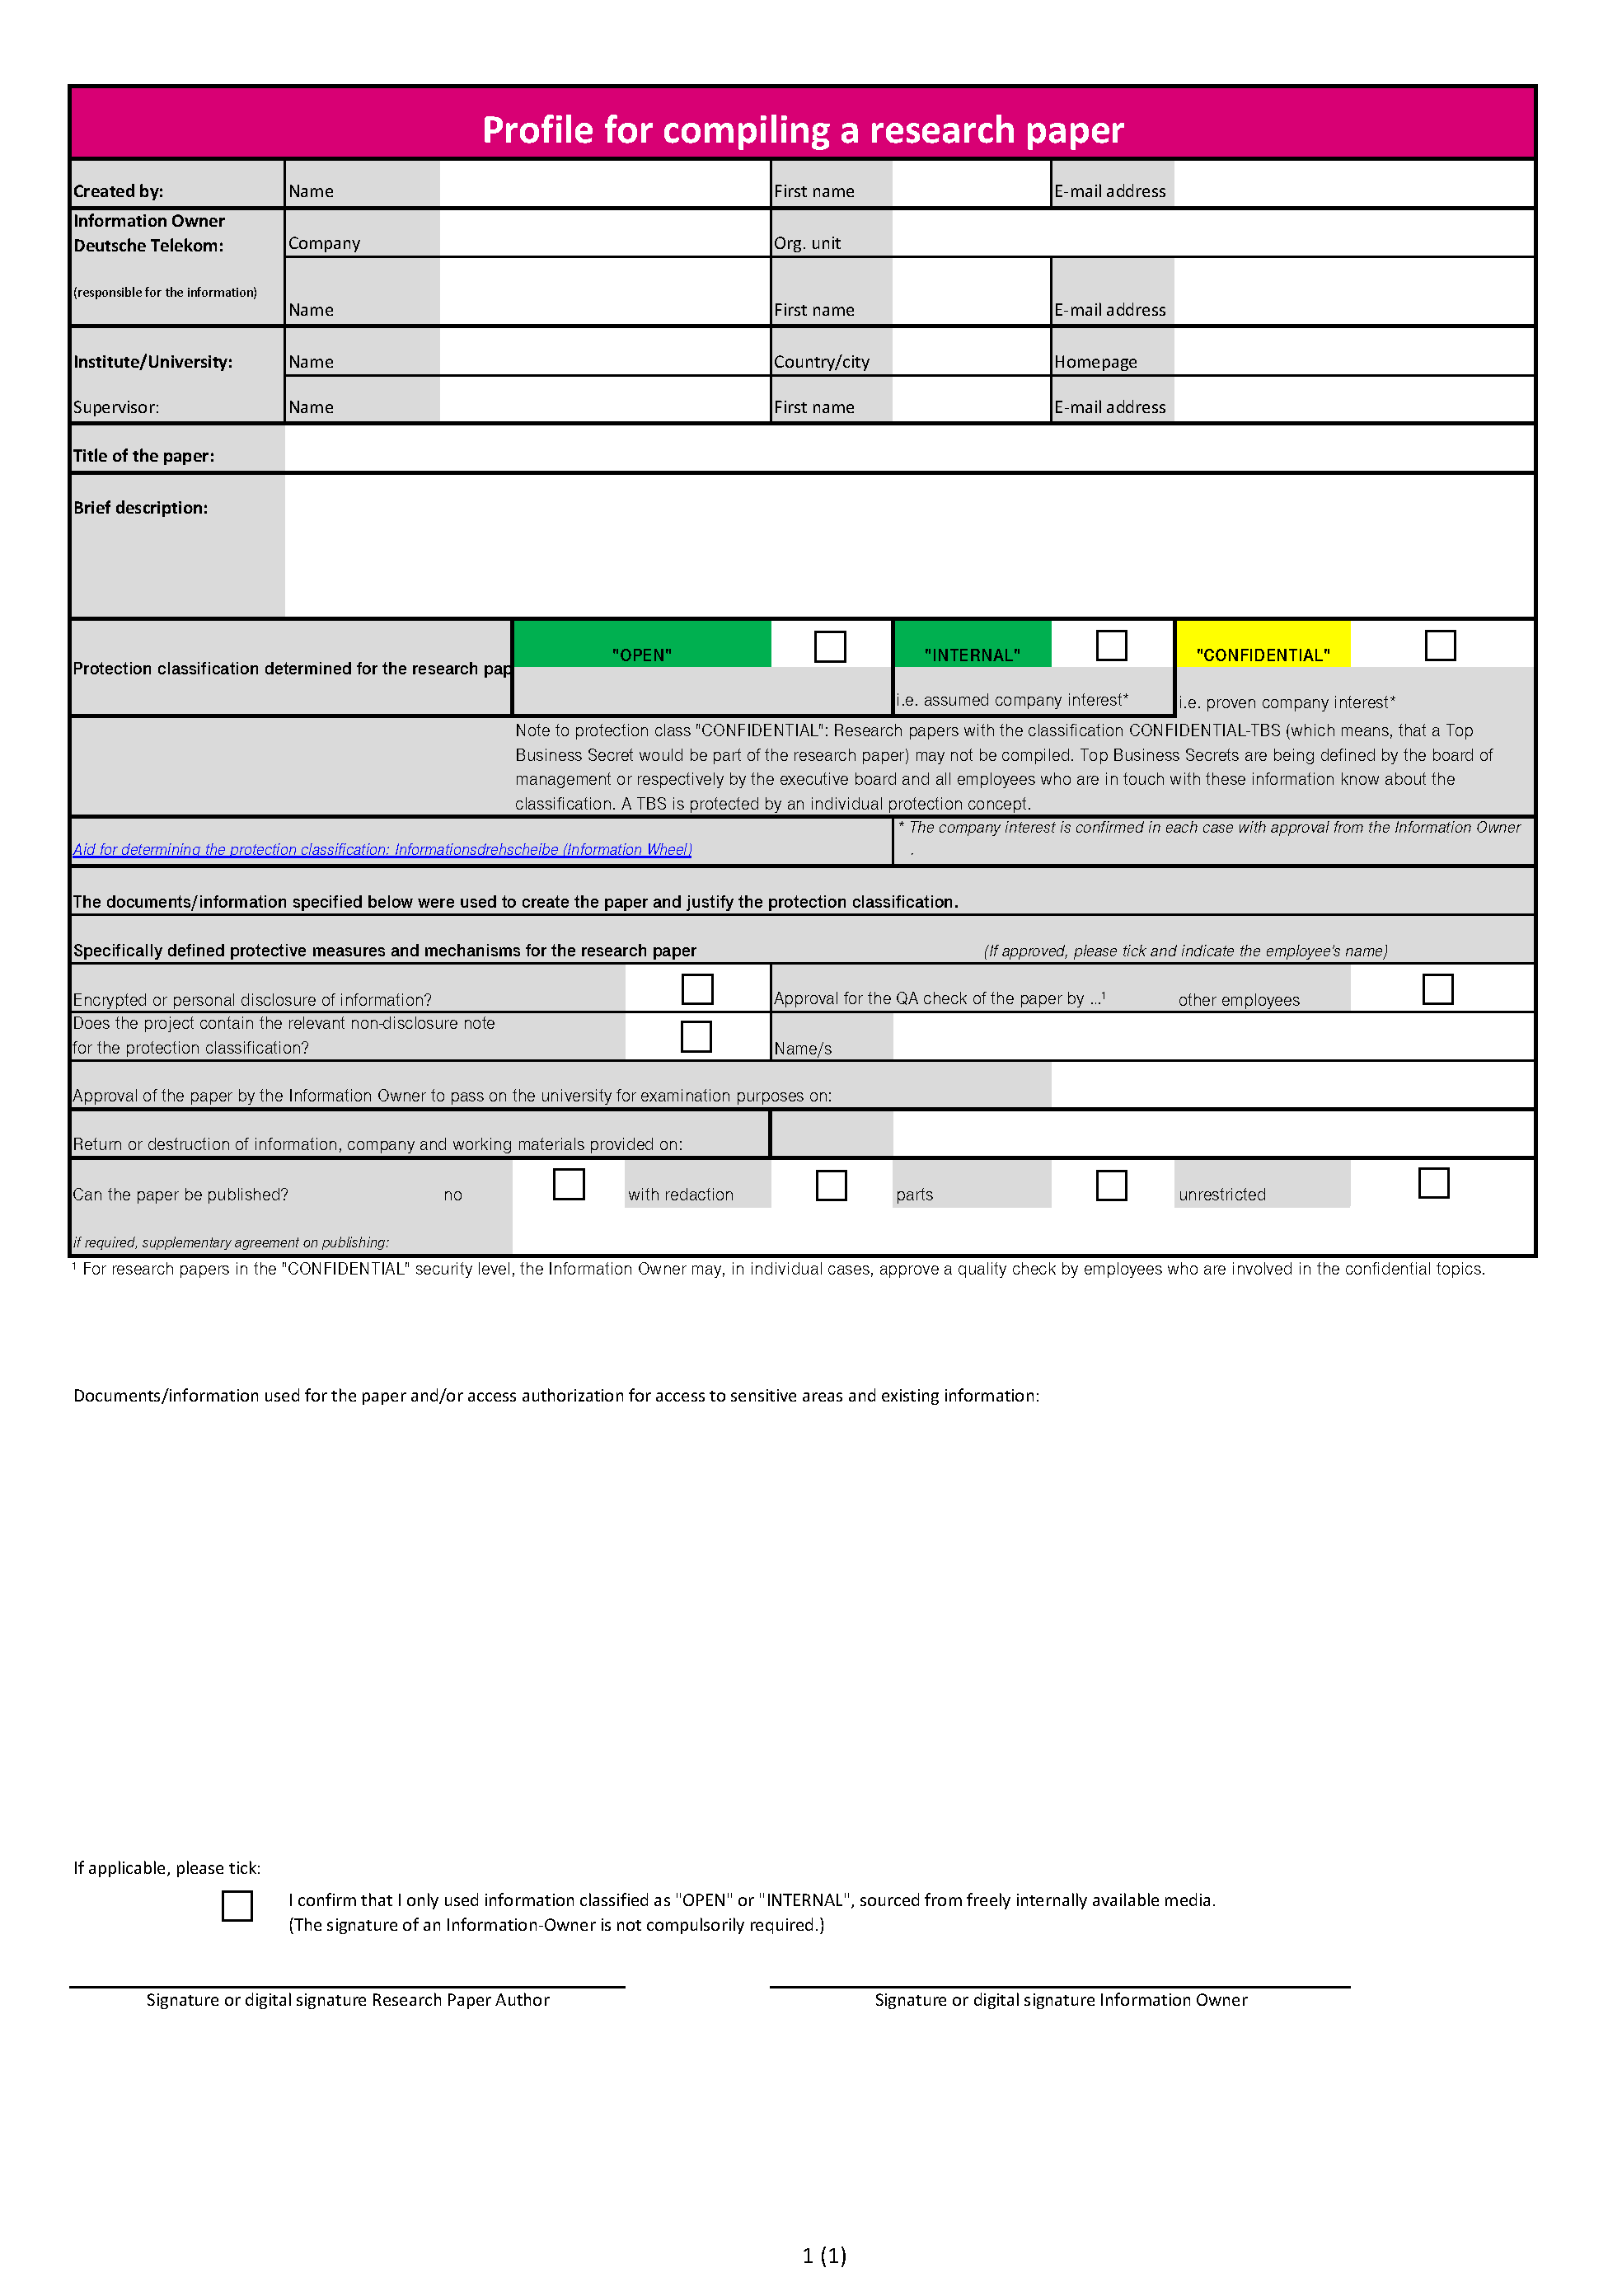
\includegraphics[width=\textwidth,height=0.95\textheight, keepaspectratio]{non-disclosure-note.pdf}
  \caption{Non-Disclosure Note}
  \label{fig:non-disclosure-note}
\end{figure}
